\documentclass[12pt]{article}
\usepackage{amsfonts, epsfig}
\usepackage[authoryear]{natbib}
\usepackage{graphicx}
\usepackage{fancyhdr}
\usepackage{amsmath}
\usepackage{xcolor}
\pagestyle{fancy}
\lfoot{\texttt{coms10013.github.io}}
\lhead{Analysis - 3.1 Taylor expansion - Conor}
\rhead{\thepage}
\cfoot{}
\begin{document}

\section*{The Taylor expansion}

We recall from our ``infinitessimal'' treatment of derivatives that
\begin{equation}
  \frac{df}{dt}=\frac{f(t+dt)-f(t)}{dt}
\end{equation}
where $dt$ is regarded in some fictional way as being a number so
small that we can set it to zero when it is convenient to do so; it is
obviously inconvenient in the definition above since that would give
zero over zero. In our previous discussion we saw how this could all
be made rigorous using the limits and epsilson-delta boxes and so on,
but we also noted how intuitively useful this picture is.

The formula can be turned around
\begin{equation}
  f(t+\delta t)\approx f(t)+f'(t)\delta t
\end{equation}
where $\delta t$ isn't an infinitessimal, just a very small number; this
is also where the formula is approximate; here for convenience later when we have lots of higher derivatives, I use $f'(t)$ rather than $\dot{f}(t)$ to denote the derivated:
\begin{equation}
  f'(t)=\left.\frac{df}{dt}\right|_t
\end{equation}
Anyway, the formula, $f(t+\delta t)\approx f(t)+f'(t)\delta t$, makes a
lot of sense, for simplicity thinking of $t$ as time the formula,
sometimes called the \textbf{Euler approximation}, says that the value
of a function after a small extra time $\delta t$ has passed, it the original value plus
delta times the rate of change; or, the change in the function is the
rate of change by the time it has spent changing. Of course, this
leaves out the possibility the rate of change is also changing. To
give an example from physics, is an object is moving at $v$ the amount
it moves after $\delta$ time is $v\delta$, but this only works if $v$
is constant.

In fact, with a bit of thought it is possible to work out formula that
takes all of this, where this is the rate of change of the rate of change, and the rate of change of that and so on, into account. This is the \textbf{Taylor expansion}: it says
\begin{equation}
  f(t+\delta t)=f(t)+f'(t)\delta t+\frac{1}{2}f''(t)\delta t^2+\frac{1}{6}f'''(t)\delta t^3+\ldots
\end{equation}
or to avoid the `$\ldots$'
\begin{equation}
  f(t+\delta t)=f(t)+\sum_{n=1}^\infty \frac{1}{n!}f^{(n)}(t)\delta t^n
\end{equation}
where
\begin{equation}
  f^{(n)}(t)=\left.\frac{d^nf}{dt^n}\right|_t
\end{equation}
and, finally, to write the same thing with different notation
\begin{equation}
  f(t+\delta t)=f(t)+\sum_{n=1}^\infty \frac{1}{n!}\left.\frac{d^nf}{dt^n}f\right|_t\delta t^n
\end{equation}
We often say this is the Taylor expansion around $t$, usually $t$ would be a specific value, so the Taylor expansion of $f(t)$ around $t=0$ would be
\begin{equation}
  f(\delta t)=f(0)+\sum_{n=1}^\infty \frac{1}{n!}f^{(n)}(0)\delta t^n
\end{equation}
or, say, around $t=2$
\begin{equation}
  f(2+\delta t)=f(2)+\sum_{n=1}^\infty \frac{1}{n!}f^{(n)}(2)\delta t^n
\end{equation}

Whatever the notation, this is a powerful and useful formula. There is
nothing very complicated about how it is derived; basically you can
get to it by applying the Euler formula to the derivative itself to
get an estimate for the average value of the derivative and then do
the same for the derivative of the derivative and so on. We don't look
at that here for reasons of time, not because it is too difficult. We
haven't said how often the Taylor expansion works; for example, $f(t)$ might have funny
behaviour, for example if $f(t)=t+1/t$ then the Taylor expansion
around $t=0$ wouldn't work and, indeed $f(t)$ goes to infinity as $t$
gets closer to zero. In that case, there is a more general version of
the Taylor expansion that works, the \textbf{Laurent series}; we don't
look at that here. We have also ignored the issue of convergence; does
the error in not doing the sum all the way to infinity get smaller as
we take more terms. It seems likely that this is the case since the
$1/n!$ term gets very large, in fact, this is not generally true,
there are functions for which the series does not work, but, again, we
are going to ignore that here and think about the large class of
well-behaved functions whose Taylor expansions are well-behaved.

In fact, there is an interesting issue here; for the class of these
well-behaved functions, called \textbf{analytic functions}, the Taylor
expansion seems to say that there are two ways to write down the
function, for a function which is analytic around $t=0$, in the first
description $f(t)$ gives a value for $f$ at each value $t$, in the
second, describes the function in terms of the derivatives, $f(0$,
$f'(0)$, $f''(0)$ and so on, with the Taylor expansion translating
from the second description back to the first. There is one of a
number examples of functions having two different descriptions,
another example is given by Fourier analysis, we won't talk more about
that here and instead just think of the Taylor expansion as a way to
approximate functions and work out properties for them.

Let's look at an example,
\begin{equation}
  f(t)=\cos{t}
\end{equation}
around $t=0$. Now $f'(t)=-\sin{t}$ and $f''(t)=-\cos{t}$ and
$f'''(t)=\sin{t}$ and $f^{(4)}(t)=\cos{t}$ and after that the cycle
repeats. Using $\sin{0}=0$ and $\cos{0}=1$ this tells us that
\begin{equation}
  \cos{t}=1-\frac{1}{2}t^2+\frac{1}{24}t^4-\frac{1}{720}t^6+\ldots
\end{equation}
We can see how well this works in Figure~1.
\begin{figure}
  \begin{center}
    % GNUPLOT: LaTeX picture with Postscript
\begingroup
  \makeatletter
  \providecommand\color[2][]{%
    \GenericError{(gnuplot) \space\space\space\@spaces}{%
      Package color not loaded in conjunction with
      terminal option `colourtext'%
    }{See the gnuplot documentation for explanation.%
    }{Either use 'blacktext' in gnuplot or load the package
      color.sty in LaTeX.}%
    \renewcommand\color[2][]{}%
  }%
  \providecommand\includegraphics[2][]{%
    \GenericError{(gnuplot) \space\space\space\@spaces}{%
      Package graphicx or graphics not loaded%
    }{See the gnuplot documentation for explanation.%
    }{The gnuplot epslatex terminal needs graphicx.sty or graphics.sty.}%
    \renewcommand\includegraphics[2][]{}%
  }%
  \providecommand\rotatebox[2]{#2}%
  \@ifundefined{ifGPcolor}{%
    \newif\ifGPcolor
    \GPcolortrue
  }{}%
  \@ifundefined{ifGPblacktext}{%
    \newif\ifGPblacktext
    \GPblacktexttrue
  }{}%
  % define a \g@addto@macro without @ in the name:
  \let\gplgaddtomacro\g@addto@macro
  % define empty templates for all commands taking text:
  \gdef\gplbacktext{}%
  \gdef\gplfronttext{}%
  \makeatother
  \ifGPblacktext
    % no textcolor at all
    \def\colorrgb#1{}%
    \def\colorgray#1{}%
  \else
    % gray or color?
    \ifGPcolor
      \def\colorrgb#1{\color[rgb]{#1}}%
      \def\colorgray#1{\color[gray]{#1}}%
      \expandafter\def\csname LTw\endcsname{\color{white}}%
      \expandafter\def\csname LTb\endcsname{\color{black}}%
      \expandafter\def\csname LTa\endcsname{\color{black}}%
      \expandafter\def\csname LT0\endcsname{\color[rgb]{1,0,0}}%
      \expandafter\def\csname LT1\endcsname{\color[rgb]{0,1,0}}%
      \expandafter\def\csname LT2\endcsname{\color[rgb]{0,0,1}}%
      \expandafter\def\csname LT3\endcsname{\color[rgb]{1,0,1}}%
      \expandafter\def\csname LT4\endcsname{\color[rgb]{0,1,1}}%
      \expandafter\def\csname LT5\endcsname{\color[rgb]{1,1,0}}%
      \expandafter\def\csname LT6\endcsname{\color[rgb]{0,0,0}}%
      \expandafter\def\csname LT7\endcsname{\color[rgb]{1,0.3,0}}%
      \expandafter\def\csname LT8\endcsname{\color[rgb]{0.5,0.5,0.5}}%
    \else
      % gray
      \def\colorrgb#1{\color{black}}%
      \def\colorgray#1{\color[gray]{#1}}%
      \expandafter\def\csname LTw\endcsname{\color{white}}%
      \expandafter\def\csname LTb\endcsname{\color{black}}%
      \expandafter\def\csname LTa\endcsname{\color{black}}%
      \expandafter\def\csname LT0\endcsname{\color{black}}%
      \expandafter\def\csname LT1\endcsname{\color{black}}%
      \expandafter\def\csname LT2\endcsname{\color{black}}%
      \expandafter\def\csname LT3\endcsname{\color{black}}%
      \expandafter\def\csname LT4\endcsname{\color{black}}%
      \expandafter\def\csname LT5\endcsname{\color{black}}%
      \expandafter\def\csname LT6\endcsname{\color{black}}%
      \expandafter\def\csname LT7\endcsname{\color{black}}%
      \expandafter\def\csname LT8\endcsname{\color{black}}%
    \fi
  \fi
    \setlength{\unitlength}{0.0500bp}%
    \ifx\gptboxheight\undefined%
      \newlength{\gptboxheight}%
      \newlength{\gptboxwidth}%
      \newsavebox{\gptboxtext}%
    \fi%
    \setlength{\fboxrule}{0.5pt}%
    \setlength{\fboxsep}{1pt}%
    \definecolor{tbcol}{rgb}{1,1,1}%
\begin{picture}(5040.00,3440.00)%
    \gplgaddtomacro\gplbacktext{%
      \csname LTb\endcsname%%
      \put(616,769){\makebox(0,0)[r]{\strut{}$-1$}}%
      \csname LTb\endcsname%%
      \put(616,1351){\makebox(0,0)[r]{\strut{}$-0.5$}}%
      \csname LTb\endcsname%%
      \put(616,1934){\makebox(0,0)[r]{\strut{}$0$}}%
      \csname LTb\endcsname%%
      \put(616,2516){\makebox(0,0)[r]{\strut{}$0.5$}}%
      \csname LTb\endcsname%%
      \put(616,3099){\makebox(0,0)[r]{\strut{}$1$}}%
      \csname LTb\endcsname%%
      \put(789,448){\makebox(0,0){\strut{}$-\pi$}}%
      \csname LTb\endcsname%%
      \put(1747,448){\makebox(0,0){\strut{}$-\pi/2$}}%
      \csname LTb\endcsname%%
      \put(2706,448){\makebox(0,0){\strut{}$0$}}%
      \csname LTb\endcsname%%
      \put(3664,448){\makebox(0,0){\strut{}$\pi/2$}}%
      \csname LTb\endcsname%%
      \put(4622,448){\makebox(0,0){\strut{}$\pi$}}%
    }%
    \gplgaddtomacro\gplfronttext{%
      \csname LTb\endcsname%%
      \put(2705,142){\makebox(0,0){\strut{}$t$}}%
      \csname LTb\endcsname%%
      \put(3818,3032){\makebox(0,0)[r]{\strut{}$\cos{t}$}}%
      \csname LTb\endcsname%%
      \put(3818,2828){\makebox(0,0)[r]{\strut{}two terms}}%
      \csname LTb\endcsname%%
      \put(3818,2624){\makebox(0,0)[r]{\strut{}three terms}}%
      \csname LTb\endcsname%%
      \put(3818,2420){\makebox(0,0)[r]{\strut{}four terms}}%
    }%
    \gplbacktext
    \put(0,0){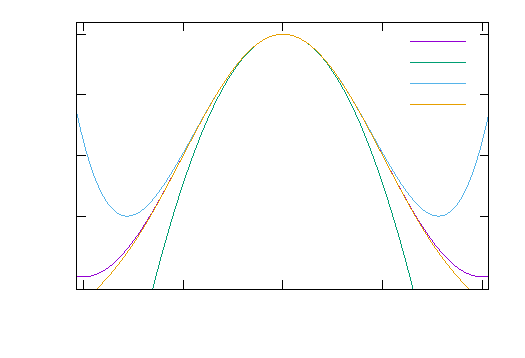
\includegraphics[width={252.00bp},height={172.00bp}]{cos}}%
    \gplfronttext
  \end{picture}%
\endgroup

    \end{center}
  \caption{A comparison of $\cos{t}$ with successive terms of Taylor expansion; we see the approximation getting better and better, at least in the range we are looking at; the labelling of the terms is the number of non-zero terms included.}
\end{figure}

\section*{Summary}
The main thing to remember is the expansion itself:
\begin{equation}
  f(t+\delta t)=f(t)+\sum_{n=1}^\infty \frac{1}{n!}f^{(n)}(t)\delta t^n
\end{equation}


\end{document}

